% This is samplepaper.tex, a sample chapter demonstrating the
% LLNCS macro package for Springer Computer Science proceedings;
% Version 2.20 of 2017/10/04
%
\documentclass[runningheads]{llncs}
%
\usepackage{graphicx}
% Used for displaying a sample figure. If possible, figure files should
% be included in EPS format.
\usepackage{tikz}
\usetikzlibrary{arrows}
\usepackage{verbatim}
\usepackage{algorithm}
\usepackage[noend]{algpseudocode}
\usepackage{amssymb}
\usepackage{amsfonts}
\usepackage{amsmath}
\let\proof\relax\let\endproof\relax
\usepackage{amsthm}
\usepackage{graphicx}
%\usepackage[all]{xy}
\usepackage{array}
\usepackage{enumitem}
%\usepackage{cite}
\usepackage[numbers]{natbib}
\usepackage{wrapfig}
\usepackage{multirow}
\theoremstyle{definition}
\renewcommand{\qedsymbol}{\hfill\ensuremath{\blacksquare}}
%\newtheorem{definition}{Definition}[section]
% If you use the hyperref package, please uncomment the following line
% to display URLs in blue roman font according to Springer's eBook style:
% \renewcommand\UrlFont{\color{blue}\rmfamily}
\usepackage[breaklinks=true]{hyperref}
\usepackage{breakcites}
\renewcommand\UrlFont{\color{blue}\rmfamily}

\input{lib/coq-listings}

%%% added lib and commands
\newcommand{\squash}{\itemsep=0pt\parskip=0pt}
\input{prelude.tex}
\usepackage{varwidth}
%\usepackage{minted}
%\usepackage{tcolorbox}
\usepackage{caption}

\newcolumntype{M}[1]{>{\centering\arraybackslash}m{#1}}
\newcolumntype{N}{@{}m{0pt}@{}}

\begin{document}
%
\title{An Ordering over Attestation Protocols\thanks{This work is
    funded in part by the NSA Science of Security initiative contract
    \#H98230-18-D-0009 and Honeywell FMT Purchase Order
    \#N000422909. The views and conclusions contained in this document
    are those of the authors and should not be interpreted as
    representing the official policies, either expressed or implied,
    of the U.S. Government.}
}
%
%\titlerunning{Abbreviated paper title}
% If the paper title is too long for the running head, you can set
% an abbreviated paper title here
%
\author{Anna Fritz \and
Sarah Johnson \and
Perry Alexander}
%
\authorrunning{A. Fritz et al.}
% First names are abbreviated in the running head.
% If there are more than two authors, 'et al.' is used.
%
\institute{Institute for Information Sciences \\ The
  University of Kansas \\ Lawrence, KS 66045 \\
  \email{\{arfritzz,sarahjohnson,palexand\}@ku.edu}}
%
\maketitle              % typeset the header of the contribution
%
\begin{abstract}
Semantic remote attestation is a process of obtaining verifiable
evidence from a remote party to establish trust. A relying party makes
a request of a target in the form of an attestation protocol that
produces evidence for appraisal. The appraisal result determines if
and how the relying party will continue interactions with the
target. This process occurs within the presence of adversaries intent
on misleading the relying party to trust a system they should
not. This research introduces a robust approach to evaluating and
comparing attestation protocols based on their resilience against such
adversaries. We develop a Coq-based, formally-verified mathematical
model aimed at quantifying the difficulty for an active adversary to
successfully compromise the protocol. Our model allows us to
systematically rank attestation protocols by the level of adversary
effort required to produce misleading evidence that does not
accurately reflect the target system's state. 

\keywords{remote attestation \and formal verification \and protocol ordering.}
\end{abstract}
%
%
%
\section{Introduction}

\emph{Semantic remote
  attestation}\citep{Haldar:04:Semantic-Remote,coker2011principles} is
a process of obtaining verifiable evidence from a remote party to
establish trust.  A \emph{relying party} makes a request of a
\emph{target} that produces evidence for \emph{appraisal}. The
appraisal result determines if and how the relying party will continue
interactions with the target.  \citet{Coker::Principles-of-R}~define
an attestation process centered on the execution of \emph{attestation
  protocols} by \emph{attestation managers}.  An attestation protocol
is a sequence of: (i) locally performed measurements; (ii) signing and
hashing data; and (iii) attestation requests sent to other parties.
We have since defined Copland~\citep{Rowe:2019:Orchestrating}, a
formally specified domain specific language for attestation protocols
and the maat~\citep{Pendergrass:2018:Maat} and
MAESTRO~\citep{Petz:2021:faithful} infrastructures implementing
Copland protocol execution.

When designing or selecting attestation protocols it is critical that
we know when one protocol is ``better'' than another.
\citet{Fritz:2023:framework} provide a framework for protocol
negotiation that defines protocol \emph{soundness} and
\emph{sufficiency}.  Here we examine \emph{protocol ordering}, an
important concept related to sufficiency that defines when one
protocol is objectively better than another.  The goal of attestation
is evaluating trust by executing protocols that gather and appraise
evidence.  The adversary's goal is to hide bad behavior by avoiding or
compromising attestation.  Our objective becomes choosing an
attestation protocol that makes the adversary's job as difficult as
possible.

Our protocol ordering makes several assumptions. First, we consider an
active adversary that is capable of corrupting any component of the
target causing it to deviate from its regular behavior.  Similarly the
adversary is capable of repairing any component of the target it
corrupts returning it to its regular behavior. Thus, a corruption
event followed by a repair event results in a component that is
indistinguishable from the original component and therefore
measurement misses the corruption. The one exception is the target's
root-of-trust for measurement (RTM) component that we assume cannot be
corrupted or repaired.

We assume an adversary will choose the easiest available attack
allowed by a protocol. Therefore, a better protocol increases the
demands of an adversary by making the easiest attack more
difficult. For an adversary to attack an attestation protocol means to
corrupt and repair a target system's components in a manner that
passes appraisal and therefore evades detection.  We assume a good
measurer invoked by an attestation protocol will generate evidence
that accurately reflects the corruption state of its target.  A
corrupt measurer or a measurer dependent on a corrupt component will
always generate evidence that indicates a good target regardless of
the target's actual state.  Finally, our analysis relies solely on the
structure of protocols and possible attacks and is agnostic to the
specific details of how an adversary can corrupt or repair system
components.

% Considering these assumptions, the formalized model and subsequent analysis support the following two principles.

% \begin{enumerate}
%     \item Measurements that mimic the system's dependency chain better confine the adversary
%     \item Increasing the number of measurements does not necessarily further confine the adversary 
% \end{enumerate}



\section{Preliminaries}

Properties of orderings and the Chase model finder developed by MITRE
\cite{Ramsdell:2020:Chase} are primary tools for our protocol ordering
and subsequent analysis. Key concepts include equivalence and partial
order relations and Chase generated attack trees.

\subsection*{Properties of Orders}

Critical to our study are the canonical properties of a binary
relation $R$ over a set $X$. We use the following
properties:

\begin{itemize}
  \squash
\item \emph{reflexive} -- $ \forall\: x\: \in X$, $R\: x\: x$
\item \emph{irreflexive} -- $ \forall \: x\: \in X, \: \neg \: R\: x\: x$
\item \emph{symmetric} -- $ \forall\: x\: , y\: \in X,$ $R\: x\: y\:\rightarrow R\: y\: x$
\item \emph{asymmetric} --  $\forall\: x,\: y\:\in X,\: R\: x\: y\:\: \rightarrow  \:\: \neg \:R\: y\: x $  
\item \emph{antisymmetric} --  $\forall\: x,\: y\:\in X,\: R\: x\: y\:\: \rightarrow \:\: R\: y\: x \rightarrow \:x = y$ 
\item \emph{transitive} -- $ \forall\: x,\: y,\: z\:\in X$, $R\: x\: y\: \rightarrow R\: y\: z \rightarrow R\: x\: z$
\end{itemize}

\noindent These properties are subsequently used to define ordering relations:

\begin{itemize}
  \squash
\item a \emph{preorder} is reflexive and transitive
\item an \emph{equivalence} relation is reflexive, symmetric, and transitive 
\item a \emph{partial order} is reflexive, antisymmetric, and transitive 
\item a \emph{strict partial order} is irreflexive, asymmetric, and transitive 
\end{itemize}

\subsection*{Chase Analysis}

Chase \cite{Ramsdell:2020:Chase,Rowe:2021:AutomatedTrust} is a first
order model finder that utilizes geometric
logic~\citep{Enderton:logic} to find minimal models of a given
theory. Inputs to the Chase model finder include a set of axioms
describing assumptions and system dependencies. From those axioms,
Chase generates all satisfying

%% TODO: Talk about difference between these attack trees and those used in the security field

\citet{Rowe:2021:AutomatedTrust}~define a Chase model for Copland
attestation protocols useful for establishing the susceptibility of a
protocol to attack. Given a Copland phrase, a model of adversary
events, and a model of the evaluated protocol, Chase produces output
enumerating all possible protocol executions as attack trees. These
sequential attack trees~\citep{Horne:Attack, Jhaware:attack} are
formal models of adversary attacks that evade detection by the
attestation protocol.  In an attack trees the presence of an active
adversary can be recognized by the corruption and repair of target
system components. The specific details of how an adversary performs
corruption and repair are not the focus of this work nor of
Chase. Instead, the goal of Chase is to allow users to better
understand potential vulnerabilities of the Copland
protocol itself.

Consider a trivial example Copland protocol where two measurements are
performed in sequence: \texttt{ms1} \texttt{+<+} \texttt{ms2}.
The measurement \texttt{ms1} is performed followed by the
final measurement \texttt{ms2}. In this abstract scenario, \texttt{ms1} and
\texttt{ms2} depend on some components of the environment, namely
\texttt{c1} and \texttt{c2}; additionally \texttt{ms1} depends on
\texttt{c3}. These system dependencies are realized within the
user-defined theory file input into the Chase model finder. Running
Chase on this protocol generates attack trees as found in Figure
\ref{fig:chase-ex}. In these figures, the prefix \texttt{ms}
represents measurement events with final measurement events presented
within green boxes. The prefixes \texttt{c\_} and  \texttt{r\_} 
represent the corruption and repair of components. Both
corruption and repair events are classified as adversary events and
are presented within yellow and orange boxes respectively. Arrows 
represent chronological time. This abstract labeling scheme mirrors that of the Chase output.

\begin{figure}[hbtp]
    \centering 
    \begin{tabular}{m{3cm} m{3cm} m{3cm}}
        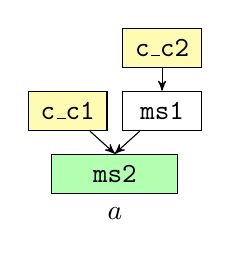
\begin{tikzpicture}[->,>=stealth']

    \node[rectangle,
          draw,
          fill = green!30,
          minimum width = 1.6cm, 
          minimum height = 0.5cm
          ] (ms4) at (0,0) {};
    \node[] at (ms4.center) {\texttt{ms2}};

    \node[rectangle,
        draw,
        minimum width = 1cm, 
        minimum height = 0.5cm
        ] (ms2) at (.6,.8) {};
    \node[] at (ms2.center) {\texttt{ms1}};


    \node[rectangle,
        draw,
        fill = yellow!30,
        minimum width = 1cm, 
        minimum height = 0.5cm
        ] (sys) at (-.6,.8) {};
    \node[] at (sys.center) {\texttt{c\_c1}};

    \node[rectangle,
        draw,
        fill = yellow!30,
        minimum width = 1cm, 
        minimum height = 0.5cm
        ] (vc) at (.6,1.6) {};
    \node[] at (vc.center) {\texttt{c\_c2}};

    \node[rectangle,
        minimum width = 1cm, 
        minimum height = 0.5cm
        ] (label) at (0,-.5) {};
    \node[] at (label.center) {$a$};


    \path[every node/.style={font=\sffamily\small}]
    %host1 path
    (vc) edge [] node [right] {} (ms2.north) 
    (sys) edge [] node [right] {} (ms4.north)
    (ms2) edge [] node [right] {} (ms4.north) ;


\end{tikzpicture} & 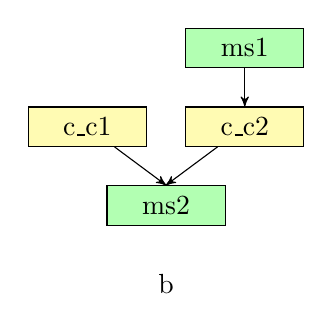
\begin{tikzpicture}[->,>=stealth']

    \node[rectangle,
          draw,
          fill = green!30,
          minimum width = 1.5cm, 
          minimum height = 0.5cm
          ] (ms4) at (0,0) {};
    \node[] at (ms4.center) {ms2};

    \node[rectangle,
        draw,
        fill = green!30,
        minimum width = 1.5cm, 
        minimum height = 0.5cm
        ] (ms2) at (1,2) {};
    \node[] at (ms2.center) {ms1};


    \node[rectangle,
        draw,
        fill = yellow!30,
        minimum width = 1.5cm, 
        minimum height = 0.5cm
        ] (sys) at (-1,1) {};
    \node[] at (sys.center) {c\_c1};

    \node[rectangle,
        draw,
        fill = yellow!30,
        minimum width = 1.5cm, 
        minimum height = 0.5cm
        ] (vc) at (1,1) {};
    \node[] at (vc.center) {c\_c2};

    \node[rectangle,
        minimum width = 1cm, 
        minimum height = 0.5cm
        ] (label) at (0,-1) {};
    \node[] at (label.center) {b};


    \path[every node/.style={font=\sffamily\small}]
    %host1 path
    (vc) edge [] node [right] {} (ms4.north) 
    (sys) edge [] node [right] {} (ms4.north)
    (ms2) edge [] node [right] {} (vc.north) ;


\end{tikzpicture} & 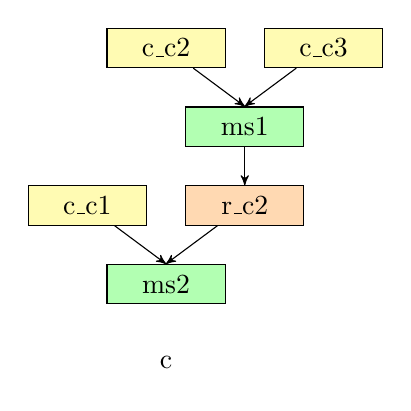
\begin{tikzpicture}[->,>=stealth']

    \node[rectangle,
          draw,
          fill = green!30,
          minimum width = 1.5cm, 
          minimum height = 0.5cm
          ] (ms4) at (0,-1) {};
    \node[] at (ms4.center) {ms2};

    \node[rectangle,
        draw,
        fill = green!30,
        minimum width = 1.5cm, 
        minimum height = 0.5cm
        ] (ms2) at (1,1) {};
    \node[] at (ms2.center) {ms1};


    \node[rectangle,
        draw,
        fill = yellow!30,
        minimum width = 1.5cm, 
        minimum height = 0.5cm
        ] (sys) at (-1,0) {};
    \node[] at (sys.center) {c\_c1};

    \node[rectangle,
        draw,
        fill = yellow!30,
        minimum width = 1.5cm, 
        minimum height = 0.5cm
        ] (c2) at (0,2) {};
    \node[] at (c2.center) {c\_c2};

    \node[rectangle,
        draw,
        fill = yellow!30,
        minimum width = 1.5cm, 
        minimum height = 0.5cm
        ] (vc) at (2,2) {};
    \node[] at (vc.center) {c\_c3};

    \node[rectangle,
        draw,
        fill = orange!30,
        minimum width = 1.5cm, 
        minimum height = 0.5cm
        ] (r1) at (1,0) {};
    \node[] at (r1.center) {r\_c2};

    \node[rectangle,
        minimum width = 1cm, 
        minimum height = 0.5cm
        ] (label) at (0,-2) {};
    \node[] at (label.center) {c};


    \path[every node/.style={font=\sffamily\small}]
    %host1 path
    (r1) edge [] node [right] {} (ms4.north) 
    (c2) edge [] node [right] {} (ms2.north) 
    (vc) edge [] node [right] {} (ms2.north) 
    (sys) edge [] node [right] {} (ms4.north)
    (ms2) edge [] node [right] {} (r1.north) ;


\end{tikzpicture} 
    \end{tabular}
    \caption[Example Chase Models]{Example Chase models}
    \label{fig:chase-ex}
\end{figure}




\section{Overview}
We introduce a formally-verified ordering of attestation protocols by
the difficulty required for an active adversary to attack the
protocol. This ordering compares two Copland protocols by comparing
their sets of Chase-generated attack trees. Comparing sets of attack trees is reliant upon an ordering over individual attack trees.
We therefore define and verify ordering relations over both sets of attack trees and individual attack trees.

\begin{figure}[hbtp]
    \centering
    \captionsetup{justification=centering,margin=1cm}
    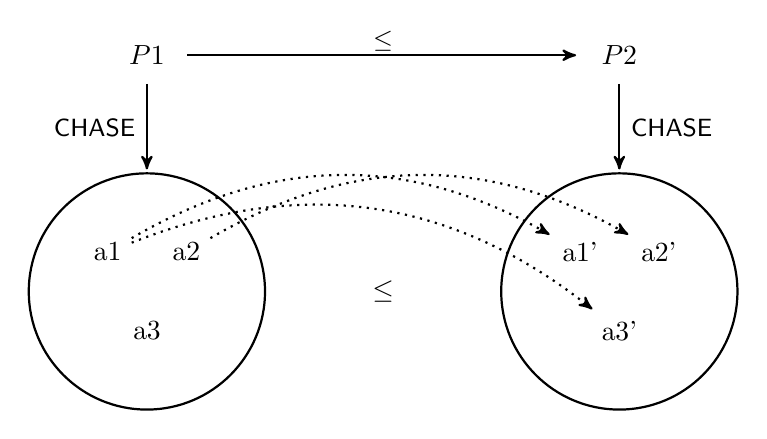
\begin{tikzpicture}[>=stealth',shorten >=1pt,auto,node distance=2.0cm,
    thick,main node/.style={rectangle,%%fill=blue!20,draw,
      font=\sffamily,minimum height=7mm,minimum width=10mm}, 
      roundnode/.style={circle, draw=black, minimum size=3cm},]
  
    \node[main node] (Phrase) {$P1$};
    %\node[main node] (ChaseP) [below of=Request] {$\langle P\rangle $};
    
    \node[main node] (Phrase') [node distance=6.0cm, right of=Phrase] {$P2$};
    % \node[main node] (ChaseP') [node distance=6.0cm, right of=Proposal] {$\langle P'\rangle$};
      
    \node[roundnode] (ChaseP) [node distance=3.0cm, below of=Phrase] {};
    \node[roundnode] (ChaseP') [node distance=6.0cm, right of=ChaseP] {};

    \node[] (a1) at (-.5,-2.5) {a1};
    \node[] (a2) at (0.5,-2.5) {a2};
    \node[] (a3) at (0,-3.5) {a3};

    \node[] (a1') at (5.5,-2.5) {a1'};
    \node[] (a2') at (6.5,-2.5) {a2'};
    \node[] (a3') at (6,-3.5) {a3'};
    %\node[] (a4') at (6.5,-3.5) {a4'};

    \node[] (ord) at (3,-3) {$\leq$};

  
    \path[every node/.style={font=\sffamily\small, fill=white,inner sep=1pt}, ->]
      (Phrase) edge node [] {$\leq$} (Phrase')
      (Phrase) edge node[left=1mm] {CHASE} (ChaseP)
      %(ChaseP) edge [dashed] node[below=1mm] {Ordering} (ChaseP')
      (Phrase') edge node[right=1mm] {CHASE} (ChaseP')
      % (a1) edge [dashed] node {} (a1')
      ;

      \draw[dotted, inner sep=0pt, ->]
        (a1) to[bend left] (a1');
      \draw[dotted, inner sep=0pt, ->]
        (a2) to[bend left] (a2');
      \draw[dotted, inner sep=0pt, ->]  
        (a1) to[bend left] (a3');
  \end{tikzpicture}
    \caption[Protocol ordering abstraction]{Diagram representing protocol ordering methodology. }
    \label{fig:protocol-org-fig}
\end{figure}

Abstractly this analysis can be visualized in Figure
\ref{fig:protocol-org-fig}.  We aim to compare two protocols $P1$ and
$P2$ to determine if $P2$ is more difficult to defeat than $P1$. To
ascertain the relationship between the two protocols, we first run
Chase to generate the set of attack trees $\{ a_1, a_2, a_3\}$ for
$P1$ and the set of attack trees $\{b_1, b_2, b_3\}$ for $P2$. We then
compare the attack trees individually, discovering ordering
relationships $a_1 \preceq b_1$, $a_2 \preceq b_2$, and
$a_1 \preceq b_3$ represented by the dotted lines. Looking at
the sets of attack trees, we can see that every attack tree in $P2$
has an attack in $P1$ that is at most as difficult. Assuming an
adversary would always perform the easiest attack to thwart an
appraiser, we conclude that $P2$ is at least as difficult to attack as
$P1$ and thus involves at least as much adversary effort as $P1$. Thus
we say $P1 \leq P2$.

We introduce four canonical ordering relations for attestation
protocol ordering where $=$ is an equivalence relation and $\le$ and
$\ge$ are partial orders. The relations are enumerated below.

\vspace*{-5mm}

\begin{align*}
1. & \text{ } P1 = P2 \\
2. & \text{ } P1 \le P2 \\
3. & \text{ } P1 \ge P2 \\
4. & \text{ } P1 \text{ and } P2 \text{ are incomparable}
\end{align*}

\noindent We choose to define the ordering in this way for several
reasons. First, we refrain from introducing four mutually exclusive
relationships (i.e., $=$, $<$, $>$, incomparable) because this results
in a drastic increase in the number of incomparable protocols. As such
we do not conclude that one protocol is strictly better than another
protocol. Although one might think we could define the relations
necessary to draw such conclusions using the irreflexive kernel
(deriving a strictly less than operator from the satisfaction of both
less than and not equal conditions), we found this was not appropriate
because the strictly less than operator would inadvertently introduce
an arbitrary ordering over adversarial corruption and repair events
where there should not be one.


These four ordering relations serve as foundational categories for our
protocol ordering. While the ordering may appear intuitive, defining
the ordering operations themselves and proving they possess the
required properties through Coq-based mechanized definitions and
proofs is challenging. Our results overcome this challenge, defining
and verifying the equivalence and partial order relations over sets of
attack trees which are built upon ordering relations over individual
attack trees. With this ordering infrastructure, one can provably
determine that one protocol is at least as good as another because it
requires at least as much adversary effort to generate seemingly
trustworthy evidence. 

Under our methodology, an ordering relationship between two Copland
protocol can be obtained by completing the following workflow as
demonstrated in Figure  \ref{fig:protocol-org-fig}: 

\begin{enumerate}
    \squash
    \item Obtain Chase output for each protocol
    \item Determine ordering relationships between the individual attack trees
    \item Leverage the individual ordering relationships to determine the ordering relationship between the sets of attack trees
    \item Link the set ordering relationship to determine protocol ordering relationship
\end{enumerate}

The following sections describe the process of introducing and
verifying an ordering for Copland protocols. In this paper,
mathematical definitions and proofs are presented manually, but
mechanized versions are completed in Coq and can be found at
\url{git@github.com:ku-sldg/protocol_ordering.git}. 


\section{Ordering Individual Attack Trees}

In this section we present orderings over attack trees. Specifically, we
introduce equivalence ($\simeq$), strict partial order ($\prec$), and
partial order ($\preceq$) relations over individual attack trees. In
future sections, these relations will be leveraged to introduce
equivalence and partial order relations over sets of attack trees.

The Chase generated attack trees presented in Figure
\ref{fig:chase-ex} can be used to describe the essential insights
applied in developing our protocol ordering. In attack tree $a_1$,
corruption events \texttt{c\_c1} and \texttt{c\_c2} occur before any
measurement events, giving the adversary an unrestricted amount
of time to perform these actions. In attack tree $a_2$, corruption
event \texttt{c\_c2} occurs between measurement events, confining the
adversary to a small-time window to perform this action. We assert
that performing the same action in a more limited time window (e.g.,
adversary event \texttt{c\_c2} in $a_2$ versus in $a_1$) is more
challenging. Since \texttt{c\_c1} is in both $a_1$ and $a_2$, we wish to conclude that $a_1$ is
strictly less work to perform by an adversary than $a_2$. Now in
attack tree $a_3$, an adversary must perform three corruption events
and one time-constrained repair event. This attack requires an
adversary to perform more work than $a_1$ as adversary events have
increased. Upon analyzing all three trees, it becomes apparent that
attack $a_1$ presents the easiest attack given the absence of
time-constrained events and the lowest number of actions required by
the adversary.  

Now we begin by formalizing a model of the Chase
generated attack trees. An attack tree is an instance of a directed graph.

\begin{definition}[Graph]
    A directed, labeled graph is a tuple $G = (N, E, \ell)$ where $N$ is a finite set of nodes, $E \subseteq N \times N$ is a finite set of directed edges represented as ordered pairs of nodes, and $\ell : N \rightarrow L$ is a labeling function from nodes to some set $L$ of labels. 
\end{definition} 
 
\noindent Looking at Figure \ref{fig:chase-ex}, one can see that each attack tree consists of a set of events, an arrow relationship mapping event to event, and an event labeling scheme disclosing the type of event (i.e., measurement, corruption, or repair).

\begin{definition}[Attack Tree]
    An attack tree is a directed, labeled graph where $N$ is a set of events, $E$ is a set of directed edges representing chronological time between events, and $\ell$ is a labeling function from event to measurement or adversary event label.
\end{definition}

When comparing two individual attack trees, we need only consider
events that concern an adversary. It is possible for an attack tree to
contain two measurement events occurring directly in sequence; the
fact that two measurements occurred instead of one has no bearing on
the adversary. Furthermore, an adversary is not impacted by the
details of any intermediate measurement events either. Instead,
sequential measurement events and specific names of non-final
measurement events only introduce unnecessary complications in
comparing individual attack trees. Therefore, we introduce the idea of
attack tree normalization, as formally defined below. Attack tree
normalization reduces consecutive measurement events to a single
measurement event, namely the latter one, and renames all remaining
non-final measurement events to a constant label. This process results
in attack trees containing only the events and information relevant to
an adversary.  


\begin{definition}[Attack tree Normalization]
    An attack tree is in its normal form when all sequences of consecutive measurement events are reduced to only the final measurement event in the sequence and all remaining non-final measurement events are renamed to \texttt{ms}. 
\end{definition}

\begin{figure}[htbp]
  \centering 
  \begin{tabular}{c c}
      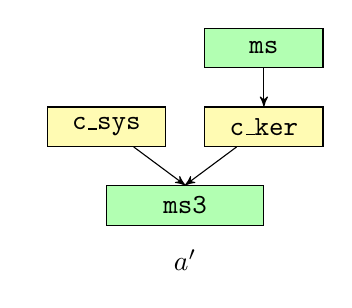
\begin{tikzpicture}[->,>=stealth']

    \node[rectangle,
          draw,
          fill = green!30,
          minimum width = 2cm, 
          minimum height = 0.5cm
          ] (ms4) at (0,0) {};
    \node[] at (ms4.center) {\texttt{ms3}};


    \node[rectangle,
        draw,
        fill = yellow!30,
        minimum width = 1.5cm, 
        minimum height = 0.5cm
        ] (sys) at (-1,1) {};
    \node[] at (sys.center) {\texttt{c\_sys}};

    \node[rectangle,
        draw,
        fill = yellow!30,
        minimum width = 1.5cm, 
        minimum height = 0.5cm
        ] (ker) at (1,1) {};
    \node[] at (ker.center) {\texttt{c\_ker}};

    \node[rectangle,
        draw,
        fill = green!30,
        minimum width = 1.5cm, 
        minimum height = 0.5cm
        ] (ms1) at (1,2) {};
    \node[] at (ms1.center) {\texttt{ms}};

    %\node[rectangle,
    %    draw,
    %    minimum width = 1.5cm, 
    %    minimum height = 0.5cm
    %    ] (ms2) at (-1,1) {};
    %\node[] at (ms2.center) {ms};

%     \node[rectangle,
%     minimum width = 1.5cm, 
%     minimum height = 0.5cm
%     ] (label) at (0,-0.5) {};
% \node[] at (label.center) {m3c};


\node[rectangle,
minimum width = 1cm, 
minimum height = 0.5cm
] (label) at (0,-.7) {};
\node[] at (label.center) {$a'$};

\node[rectangle,
minimum width = 1cm, 
minimum height = 0.5cm
] (label) at (-1.5,0) {};
\node[] at (label.center) {};


    \path[every node/.style={font=\sffamily\small}]
    %host1 path
    (ms1) edge [] node [right] {} (ker.north)
    (ker) edge [] node [right] {} (ms4.north)
    %(ms2) edge [] node [right] {} (ms4.north) 
    (sys) edge [] node [right] {} (ms4.north) ;


\end{tikzpicture} & 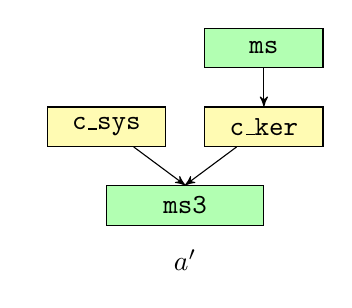
\begin{tikzpicture}[->,>=stealth']

    \node[rectangle,
          draw,
          fill = green!30,
          minimum width = 2cm, 
          minimum height = 0.5cm
          ] (ms4) at (0,0) {};
    \node[] at (ms4.center) {\texttt{ms3}};


    \node[rectangle,
        draw,
        fill = yellow!30,
        minimum width = 1.5cm, 
        minimum height = 0.5cm
        ] (sys) at (-1,1) {};
    \node[] at (sys.center) {\texttt{c\_sys}};

    \node[rectangle,
        draw,
        fill = yellow!30,
        minimum width = 1.5cm, 
        minimum height = 0.5cm
        ] (ker) at (1,1) {};
    \node[] at (ker.center) {\texttt{c\_ker}};

    \node[rectangle,
        draw,
        fill = green!30,
        minimum width = 1.5cm, 
        minimum height = 0.5cm
        ] (ms1) at (1,2) {};
    \node[] at (ms1.center) {\texttt{ms}};

    %\node[rectangle,
    %    draw,
    %    minimum width = 1.5cm, 
    %    minimum height = 0.5cm
    %    ] (ms2) at (-1,1) {};
    %\node[] at (ms2.center) {ms};

%     \node[rectangle,
%     minimum width = 1.5cm, 
%     minimum height = 0.5cm
%     ] (label) at (0,-0.5) {};
% \node[] at (label.center) {m3c};


\node[rectangle,
minimum width = 1cm, 
minimum height = 0.5cm
] (label) at (0,-.7) {};
\node[] at (label.center) {$a'$};

\node[rectangle,
minimum width = 1cm, 
minimum height = 0.5cm
] (label) at (-1.5,0) {};
\node[] at (label.center) {};


    \path[every node/.style={font=\sffamily\small}]
    %host1 path
    (ms1) edge [] node [right] {} (ker.north)
    (ker) edge [] node [right] {} (ms4.north)
    %(ms2) edge [] node [right] {} (ms4.north) 
    (sys) edge [] node [right] {} (ms4.north) ;


\end{tikzpicture} 
  \end{tabular}
  \captionsetup{justification=centering,margin=1cm}
  \caption[Example of attack tree normalization]{An example of attack tree normalization.}
  \label{fig:reduce-ex}
\end{figure}


\noindent To demonstrate attack tree normalization, consider the example presented in Figure \ref{fig:reduce-ex} where tree $a$ is normalized to $a'$. When applying attack tree normalization, the consecutive measurement events \texttt{ms2} and \texttt{ms3} are reduced to only the latter measurement event \texttt{ms3}, and the remaining non-final measurement event \texttt{ms1} is renamed to \texttt{ms}. For the remainder of this paper, unless otherwise noted, we assume all Chase-generated attack trees are in their normal form.

To compare individual Chase-generated attack trees, we introduce additional definitions to aid in determining when one attack tree requires strictly less or equivalent work to perform by an adversary. Central to this comparison is the different classification of adversary actions that may be present within an attack tree. That is, Chase generated attack trees contain measurement and adversary events, and it is the variety of consecutive occurences that may occur that influences our ordering definitions.  

\begin{definition}[Adversary Event, $\pi$]
    An adversary event is any action performed by an adversary to change the behavior of a component in a target system. Adversary events are classified as either corruption or repair events. Given an attack tree $a$, let $\pi(a) := \{n \in N_a \,|\, n \text{ is an adversary event}\,\}$. An event $n$ is an adversary event if and only if $\ell_a(n)$ is an adversary event label.
\end{definition}


As previously alluded to, time constraints escalate difficulty. That is, we assume the difficulty of an attack is increased if an adversary must complete it between measurement events. To realize this distinction, we define time-constrained adversary events formally below.  

\begin{definition}[Time-Constrained Adversary Event, $\tau$]
    A time-constrained adversary event is an adversary event where the attacker must perform the corruption or repair of a component in between measurement events thus limiting the time available to complete the action. Given an attack tree $a$, let $\tau(a) := \{n \in N_a \,|\, n \text{ is a time-constrained adversary event}\,\}$.
\end{definition}

\noindent It is worth noting that by definition, every time-constrained adversary event is itself an adversary event and therefore $\tau(a) \subseteq \pi(a)$ for every attack tree $a$.


With these preliminary definitions in place, we can now describe our proposed ordering relations. We wish to say two individual attack trees are equivalent if they are semantically equivalent. Defining equivalence in this way ensures trees that have the same adversary events in the same order and the same final measurement event are indeed equivalent, regardless of the specific, intermediate measurement events that occurred. Therefore, as stated previously, we only compare trees in their normal form so that there are no sequences of consecutive measurement events and all non-final measurement events have the same label. Now we naturally define attack tree equivalence by graph isomorphism.


\begin{definition}[Isomorphism]
    Directed, labeled graphs $G$ and $H$ are isomorphic if and only if there exists a bijection $f : N_G \to N_H$ such that for all pairs of nodes $n_1, n_2 \in N_G$, $(n_1,n_2) \in E_G$ if and only if $(f(n_1),f(n_2)) \in E_H$ and for all nodes $n \in N_G$, $\ell_G(n) = \ell_H(f(n))$.
\end{definition}


\begin{definition}[Equivalence $\simeq$]
  Attack trees $a$ and $b$ are equivalent (i.e., $a \simeq b$) if and only they are isomorphic.
\end{definition}


\noindent We formally verify that an isomorphism is an equivalence relation in Coq but do not include the mathematical proofs here since they are easily available in many textbooks or web sources. With the proofs of reflexivity, symmetry, and transitivity completed in Coq, we obtain a formally-verified equivalence relation over individual attack trees allowing us to provably determine if two trees are semantically equivalent.


Next, we must define a strict partial order relation over individual attack trees. It should be the case that under this relation one attack tree is strictly better than another if it increases the burden of an attacker. To formally define the concept of increasing adversary constraint, we analyzed many Chase-generated attack trees to ground our logic in concrete examples. By studying patterns in the trees, we select two distinct conditions that confine an adversary to consider in our ordering scheme. That is, an attack has increased difficulty if it requires more adversary events or more time-constrained adversary events. We formally define this relation below as ``strictly less work''.

\begin{definition}[Strictly Less Work]
  An attack tree $a$ requires strictly less work to perform by an adversary than attack tree $b$ if and only if at least one of the following hold: 
\begin{enumerate}
  \squash
  \item $\pi(a) \subseteq \pi(b)$ and $\tau(a) \subset \tau(b)$
  %(i.e., the set of adversary events in $a$ is subset of the set of adversary events in $b$ and the set of time-constrained adversary events in $a$ is a proper subset of the set of time-constrained adversary events in $b$)
  \item $\pi(a) \subset \pi(b)$ and $\tau(a) \subseteq \tau(b)$
  %(i.e., the set of adversary events in $a$ is a proper subset of the set of adversary events in $b$ and the set of time-constrained adversary events in $a$ is subset of the set of time-constrained adversary events in $b$)
\end{enumerate}
\end{definition}

\begin{definition}[Strict Partial Order $\prec$]
  An attack tree $a$ is strictly less than attack tree $b$ (i.e., $a \prec b$) if and only if $a$ requires strictly less work than $b$.
\end{definition}

\noindent By design, this definition only allows the comparison of attack trees $a$ and $b$ where both $\pi(a) \subseteq \pi(b)$ and $\tau(a) \subseteq \tau(b)$. In other words, we only compare attack trees that share common sets of both adversary events and time-constrained adversary events. Looking back at Figure \ref{fig:chase-ex}, we can compute the sets of adversary events and sets of time-constrained adversary events for attacks $a_1$, $a_2$, and $a_3$ and then determine what ordering relationships hold between them. For attack $a_1$ we get that $\pi(a_1) = \{ \texttt{c\_c1}, \texttt{c\_c2} \}$ and $\tau(a_1) = \emptyset$. For attack $a_2$, $\pi(a_2) = \{ \texttt{c\_c1}, \texttt{c\_c2} \}$ and $\tau(a_2) = \{ \texttt{c\_c2} \}$. And lastly for attack $a_3$, $\pi(a_3) = \{ \texttt{c\_c1}, \texttt{c\_c2}, \texttt{c\_c3}, \texttt{r\_c2} \}$ and $\tau(a_3) = \{ \texttt{r\_c2} \}$. Using the definition of strict partial order below, we can conclude that $a_1 \prec a_2$, $a_1 \prec a_3$, and $a_2$ and $a_3$ are incomparable.

Furthermore, our design of the strict partial order relation allows it to be enhanced with an ordering over adversarial events themselves. Given a strict partial order over adversarial events, it can be utilized in our definition of ``strictly less work'' in the Coq specification. This is because its definition is parameterized over an arbitrary adversary event ordering. Examples of such orderings are that corrupting a shallower component is less difficult than corrupting a deeper one and that repairing a component is less difficult than corrupting one. We do not assert that these orderings over adversarial events hold. Instead, we only provide them as examples for how our ordering scheme can be enhanced with potentially desirable considerations. For the rest of this paper, we are only reasoning under the empty relation over adversarial events, meaning we do not state that any event is more or less difficult than another.


To formally verify our strict partial order over individual attack trees is indeed a strict partial order, we prove the relation is irreflexive, asymmetric, and transitive in Coq. Our proofs rely primarily on the fact that subset is a partial order and proper subset is a strict partial order.

We additionally define a partial order relation over individual attack trees by the combination of the equivalence and strict partial order relations defined earlier in this section. This design is motivated by the reflexive closure principle. We verify in Coq that this definition is in fact a partial order by proving it is reflexive, antisymmetric, and transitive.

\begin{definition}[Partial Order $\preceq$]
  An attack tree $a$ is less than attack tree $b$ (i.e., $a \preceq b$) if and only if $a$ is isomorphic to $b$ or $a$ requires strictly less work than $b$ (i.e., $a \simeq b$ or $a \prec b$).
\end{definition}


\section{Ordering Sets of Attack Trees}

The previously introduced ordering relations over individual attack trees can be leveraged to compare protocols by ordering their corresponding sets of Chase-generated attack trees. Here, we introduce equivalence ($=$) and partial order ($\le$) relations over sets of attack trees.

First, we naturally define an equivalence relation over sets of attack trees using set equality up to isomorphism. This means that when determining one set is a subset of another, instead of requiring every element in the former to be in the latter, we only require every element in the former to be isomorphic/equivalent to an element in the latter. Mathematically, we replace the representation of $S \subseteq T$ from $\forall s \in S, s \in T$ to $\forall s \in S, \exists t \in T, s \simeq t$.

\begin{definition}[Set Equality]
  Two sets $S$ and $T$ are equal if and only $S \subseteq T$ and $T \subseteq S$.
\end{definition}

\begin{definition}[Equivalence =]
    Two sets of attack trees $P$ and $Q$ are equivalent (i.e., $P = Q$) if and only if they are equal up to isomorphism of their elements.
\end{definition}

Now before we can introduce a partial order relation, we must introduce additional infrastructure to compare sets of attack trees. We begin by recalling Rowe's definition of supports and covers below \cite{Rowe:2021:OnOrdering}.

\begin{definition}[Supports/Covers]
    Given two sets of graphs $S$ and $T$ and some preorder $R$ over graphs, we say that $S$ supports $T$ if and only if for every $h \in T$, there is some $g \in S$, such that $R\: g\: h$. We  say that $T$ covers $S$ if and only if for every $g \in S$ there is some $h \in T$ such that $R\: g\: h$.
\end{definition}

Supports states that, for every graph in $T$, there exists some related graph in $S$. Conversely, covers says that, for every graph in $S$, there exists a related graph in $T$.  This idea is best visualized by Figure \ref{fig:sup-cov} where we abstractly denote Copland protocols as $P$ and $Q$. We assume these protocols generate the corresponding sets of attack trees $\{a1, a2 , a3 \}$ and $ \{b1, b2 ,b3\}$.

\begin{figure}[htbp]
    \centering
    \usetikzlibrary{shapes.geometric}

\begin{tikzpicture}


    \node[ellipse,
    draw = black,
    minimum width = 1.5cm, 
    minimum height = 3cm] (e) at (-4.8,0) {};

    \node[ellipse,
    draw = black,
    minimum width = 1.5cm, 
    minimum height = 3cm] (e) at (-1.8,0) {};

    \node[ellipse,
    draw = black,
    minimum width = 1.5cm, 
    minimum height = 3cm] (e) at (1.8,0) {};

    \node[ellipse,
    draw = black,
    minimum width = 1.5cm, 
    minimum height = 3cm] (e) at (4.8,0) {};


    \node[] (a1) at (-4.8,.8) {$a_1$};
    \node[] (a2) at (-4.8,0) {$a_2$};
    \node[] (a3) at (-4.8,-.8) {$a_3$};

    \node[] (a1') at (-1.8,.8) {$b_1$};
    \node[] (a2') at (-1.8,0) {$b_2$};
    \node[] (a3') at (-1.8,-.8) {$b_3$};

    \node[] (b1) at (4.8,.8) {$b_1$};
    \node[] (b2) at (4.8,0) {$b_2$};
    \node[] (b3) at (4.8,-.8) {$b_3$};

    \node[] (b1') at (1.8,.8) {$a_1$};
    \node[] (b2') at (1.8,0) {$a_2$};
    \node[] (b3') at (1.8,-.8) {$a_3$};

    \node[] (label) at (-3.3, -2.1) {$S$ supports $T$};
    \node[] (label) at (3.3, -2.1) {$T$ covers $S$};

    \node[] (label) at (-4.8, 1.9) {$S$};
    \node[] (label) at (-1.8, 1.9) {$T$};

    \node[] (label) at (1.8, 1.9) {$S$};
    \node[] (label) at (4.8, 1.9) {$T$};


      \draw[->] (a1) to (a1');
      \draw[->] (a2) to (a2');
      \draw[->] (a2) to (a3');

      \draw[->] (b1') to (b1);
      \draw[->] (b2') to (b1);
      \draw[->] (b3') to (b1);
  \end{tikzpicture}
    \captionsetup{justification=centering,margin=1cm}
    \caption[Supports and covers]{A visual representation of supports and covers. \\ Arrows represent ordering relationships.}
    \label{fig:sup-cov}
\end{figure}

The definition of supports and covers is parameterized over a relation $R$. For an protocol ordering, we choose $R$ to be the partial order over attack trees defined previously. Therefore, in Figure \ref{fig:sup-cov}, arrows between the individual attack trees represent partial order relationships.

\begin{definition}[Partial Order $\leq$]
  A set of attack trees $P$ is less than a set of attack trees $Q$ (i.e., $P \leq Q$) if and only if P supports Q under the partial order relation $\preceq$.
\end{definition} 

While Rowe defines both supports and covers, we only need to be concerned with supports for our protocol ordering. The motivation for this two-fold. First, we assume that given a protocol and its associated attacks, an adversary will always perform the easiest one.
Second, we must consider our desired conclusion of protocol ordering: if a protocol $P$ is less than a protocol $Q$, then $Q$ is at least as good as $P$ and therefore \emph{should be selected over $P$}. Therefore, we must consider every attack in the better protocol so as not to overlook the easiest attack. Furthermore, we need not consider every tree in the weaker protocol. This is best understood by examining the extreme cases for the unevaluated tree: (1) it is the easiest attack or (2) it is the hardest attack. If it is the easiest attack, then clearly the protocol is still the weaker one. If it is the hardest attack, then it has no effect on the protocol since, by our assumption, an attacker would not choose this attack.

Recall that a partial order is reflexive, antisymmetric, and transitive. We easily verify in Coq that our proposed partial order relation is reflexive and transitive. Verifying that the relation is antisymmetric proved more difficult and, in fact, impossible. That is, it is impossible using the classic definition of antisymmetry (i.e., if $P \le Q$ and $Q \le P$ then $P = Q$). A simple counter example can be constructed using the attack trees in Figure \ref{fig:chase-ex}. Let $P = \{a_1,a_2\}$ and $Q = \{a_1\}$. Then $P \le Q$ since $a_1 \preceq a_1$, and $Q \le P$ since $a_1 \preceq a_1$ and $a_1 \preceq a_2$. But clearly it is not the case that $P$ is the same set as $Q$. Instead, we can see that the set of easiest attacks in $P$ is the same as the set of easiest attacks in $Q$. In fact, this property holds not only for this example but for any two protocols. Therefore, we construct and prove a modified version of antisymmetry. Before we give its precise specification, we must quantify what it means to the ``easiest'' attack.

\begin{definition}[Minimal Attack Tree, \normalfont{min}]
  An attack tree $a$ is minimal with respect to a set $P$ if and only $b \nprec a$ for every $b \in P$. Given a set of attack trees $P$, let $\text{min}(P) := \{a \in P \,|\, a \text{ is minimal with respect to } P \}$.
\end{definition}

\begin{lemma}[Minimal Set is Less than Full Set]
  For every set of attack trees $P$, $\text{min}(P) \le P$ (i.e., $\forall a \in P, \exists b \in \text{min}(P), b \preceq a$).
\end{lemma}

\begin{lemma}[Minimal Attack is Not Strictly Less than Another]
  For every set of attack trees $P$ and attack trees $a_1, a_2 \in \text{min}(P)$, $a_1 \nprec a_2$.
\end{lemma}

Our revised version of antisymmetry is stated as follows: if $P \le Q$ and $Q \le P$ then $\text{min}(P) = \text{min}(Q)$. Although this property is mathematically weaker than its standard version, it is, in practice, considering our goals, adequately and equally as strong. To prove this antisymmetry property, we must apply several facts regarding minimal attack trees provided above. These lemmas are true by the definition of minimal.



\begin{theorem}[Antisymmetry of Partial Order $\leq$]
  For all sets of attack trees $P$ and $Q$, if $P \le Q$ and $Q \le P$ then $\text{min}(P) = \text{min}(Q)$. 
\end{theorem}
\begin{proof}
  Let $P$ and $Q$ be arbitrary sets of attack trees. Suppose that $P \le Q$ and $Q \le P$. 
  
  Let us begin by proving two intermediate statements regarding the ordering relationships between $\text{min}(P)$ and $\text{min}(Q)$, namely that $\text{min}(P) \leq \text{min}(Q)$ and $\text{min}(Q) \leq \text{min}(P)$. Since $\text{min}(P) \leq P$ by Lemma 1 and $P \leq Q$ by assumption, $\text{min}(P) \leq Q$ by transitivity of $\leq$. Then since $\text{min}(Q) \subseteq Q$, $\text{min}(P) \leq \text{min}(Q)$ trivially. We can apply a similar reasoning to get that $\text{min}(Q) \leq \text{min}(P)$.

  Now recall our definition of set equivalence: $\text{min}(P) = \text{min}(Q)$ if and only if $\text{min}(P) \subseteq \text{min}(Q)$ and $\text{min}(Q) \subseteq \text{min}(P)$ up to isomorphism. Therefore, let us proceed by proving the first subgoal: $\text{min}(P) \subseteq \text{min}(Q)$ up to isomorphism (i.e., $\forall a \in \text{min}(P), \exists b \in \text{min}(Q), a \simeq b)$.  Let $a$ be an arbitrary attack tree in $\text{min}(P)$. 

  Since $\text{min}(Q) \leq \text{min}(P)$, there exists some attack tree $b \in \text{min}(Q)$ such that $b \preceq a$. Therefore, either $b \simeq a$ or $b \prec a$. Suppose $b \simeq a$. Then $a \simeq b$ by symmetry of $\simeq$. And we have proven our goal and are done. Now suppose $b \prec a$. Since $\text{min}(P) \leq \text{min}(Q)$, there exists some attack $a' \in \text{min}(P)$ such that $a' \preceq b$. Then $a' \prec a$ by transitivity of the composition of $\preceq$ and $\prec$. A contradiction by Lemma 2. Therefore, we have proven that $\text{min}(P) \subseteq \text{min}(Q)$ up to isomorphism.
  
  We can apply a similar reasoning to prove the second subgoal: $\text{min}(Q) \subseteq \text{min}(P)$ up to isomorphism. Thereby proving antisymmetry of $\leq$.
\end{proof}


With verified equivalence and partial order relations, we can link the ordering decision over sets of attack trees to their corresponding protocols allowing us to provably state that one protocol is at least as difficult to attack as another protocol. If no ordering relation holds, the protocols are incomparable. Therefore, we have formally specified and verified the four proposed ordering relations over Copland protocols. 

\section{Representative Examples}

This research finds inspiration in real-life instances of Copland protocol analysis documented in the attestation literature \cite{Rowe:2021:OnOrdering,Coker::Principles-of-R}. We ground our formally-verified protocol ordering methodology in reality by reasoning about an enterprise that would like to ensure a remote server (target) connecting to its network provides a fresh system scan by the appropriate virus checking software. Adapted from Rowe's \cite{Rowe:2016:Confining} example, the target's infrastructure consists of a platform dependent on a hardware root of trust for measurement $rtm$. Within this platform are several components, namely the kernel $ker$, a hypervisor $hv$, a virus checker $vc$, and the collective parts of the system scanned by the virus checker $sys$. The virus checker and the system are both dependent on the kernel, while the kernel and the hypervisor have no dependencies within the platform. Each component is equipped with measurement capabilities. We use the notation \texttt{ms}$(c_1,c_2)$ to denote the measurement of component $c_2$ by component $c_1$.

We select and evaluate three Copland protocols under this attestation goal and infrastructure using our protocol ordering methodology in order to demonstrate two hypotheses: (1) measurements that mimic the system's dependency chain better confine the adversary and (2) increasing the number of measurements does not necessarily further confine the adversary. Each protocol contains the same final measurement event \texttt{ms}$(vc,sys)$ since the primary goal of the enterprise is to receive a fresh system scan by the virus checker. Additionally, each protocol contains the same penultimate measurement event \texttt{ms}$(ker,vc)$ since an ancillary goal of the enterprise is to determine whether the target is running the appropriate virus checker.

%%% NOTE: Uses true Copland syntax
% \begin{table}[h]
%   \setlength\extrarowheight{7pt}
%   \centering
%   \footnotesize
%   \begin{tabular}{|M{2.2cm}|M{9.7cm}|N}
%       \hline
%       Protocol Name & Actual protocol &\\
%       \hline   
%       $ker\text{-}vc\text{-}sys$ & *target:  $\at{\texttt{p4}}{(\texttt{ker p4 vc})}$ \texttt{+<+} $\at{\texttt{p4}}{(\texttt{vc p4 sys})}$ &\\ \hline 
%       $rtm\text{-}ker\text{-}vc\text{-}sys$ & *target: $\at{\texttt{p1}}{(\texttt{rtm p4 ker})}$ \texttt{+<+} $\at{\texttt{p4}}{(\texttt{ker p4 vc})}$ \texttt{+<+} $\at{\texttt{p4}}{(\texttt{vc p4 sys})}$ &\\
%       \hline
%       $ker\text{-}hv\text{-}vc\text{-}sys$ & *target: $\at{\texttt{p4}}{(\texttt{ker p4 hv})}$ \texttt{+<+} $\at{\texttt{p4}}{(\texttt{ker p4 vc})}$ \texttt{+<+} $\at{\texttt{p4}}{(\texttt{vc p4 sys})}$ &\\ \hline 
%   \end{tabular}
%   \caption[Chase Analysis with Varied Dependencies]{Example Copland protocols analyzed with Chase}
%   \label{Chase-table}
% \end{table}

%% NOTE: Uses abstract Copland syntax
\begin{table}[h]
  \setlength\extrarowheight{7pt}
  \centering
  \footnotesize
  \begin{tabular}{|M{1cm}|M{8cm}|N}
      \hline  
      $P1$ & *target:  \texttt{ms}$(ker, vc)$ \texttt{+<+} \texttt{ms}$(vc, sys)$ &\\ \hline 
      $P2$ & *target: \texttt{ms}$(rtm, ker)$ \texttt{+<+} \texttt{ms}$(ker, vc)$ \texttt{+<+} \texttt{ms}$(vc, sys)$ &\\
      \hline
      $P3$ & *target: \texttt{ms}$(ker, hv)$ \texttt{+<+} \texttt{ms}$(ker, vc)$ \texttt{+<+} \texttt{ms}$(vc, sys)$ &\\ \hline 
  \end{tabular}
  \caption[Chase Analysis with Varied Dependencies]{Abstractly rendered Copland protocols}
  \label{Chase-table}
\end{table}


The first protocol $P1$ is our baseline protocol consisting only of the required measurement events described above. The second protocol $P2$ is intended to strengthen the first by prepending the measurement event \texttt{ms}$(rtm,ker)$. Since the virus checker and system depend on the kernel, taking a measurement of the kernel from a trusted place should strengthen the protocol according to hypothesis 1. The third protocol $P3$ is intended to be no stronger than the first by prepending the measurement event \texttt{ms}$(ker,hv)$. Since the virus checker and system are independent of the hypervisor, taking a measurement of the hypervisor should not change the strength of the protocol according to hypothesis 2. We apply our protocol ordering to these protocols to verify that this reasoning does indeed hold.

\begin{figure}[h]
    \begin{center}
        \begin{tabular}{ M{6cm} | M{6cm} }
                $P1$ & $P2$ \\
                \hline
                &\\ 
                \input{examples/ker_vs-sys-seq_reduced-copy/m1.tex} \hspace{.03cm} 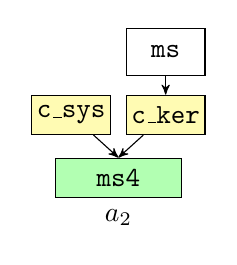
\begin{tikzpicture}[->,>=stealth']

    \node[rectangle,
          draw,
          fill = green!30,
          minimum width = 1.6cm, 
          minimum height = 0.5cm
          ] (ms4) at (0,0) {};
    \node[] at (ms4.center) {\texttt{ms4}};

    \node[rectangle,
    minimum width = 1cm, 
    minimum height = 0.5cm
    ] (lab) at (0,-.5) {};
  \node[] at (lab.center) {$a_2$};

    \node[rectangle,
        draw,
        fill = yellow!30,
        minimum width = 1cm, 
        minimum height = 0.5cm
        ] (sys) at (-.6,.8) {};
    \node[] at (sys.center) {\texttt{c\_sys}};

    \node[rectangle,
        draw,
        fill = yellow!30,
        minimum width = 1cm, 
        minimum height = 0.5cm
        ] (vc) at (.6,.8) {};
    \node[] at (vc.center) {\texttt{c\_ker}};

    \node[rectangle,
        draw,
        minimum width = 1cm, 
        minimum height = 0.6cm
        ] (ms3) at (.6,1.6) {};
    \node[] at (ms3.center) {\texttt{ms}};

%     \node[rectangle,
%     minimum width = 1cm, 
%     minimum height = 0.5cm
%     ] (label) at (0,-0.5) {};
% \node[] at (label.center) {m2b};


    \path[every node/.style={font=\sffamily\small}]
    %host1 path
    (ms3) edge [] node [right] {} (vc.north)
    (vc) edge [] node [right] {} (ms4.north) 
    (sys) edge [] node [right] {} (ms4.north) ;


\end{tikzpicture} 
                & \input{examples/rtm_ker-vc-sys-seq_reduced-copy/m1.tex} \hspace{.03cm} 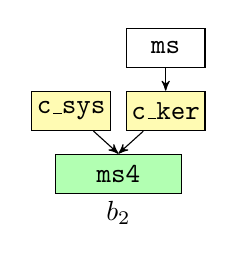
\begin{tikzpicture}[->,>=stealth']

    \node[rectangle,
          draw,
          fill = green!30,
          minimum width = 1.6cm, 
          minimum height = 0.5cm
          ] (ms4) at (0,0) {};
    \node[] at (ms4.center) {\texttt{ms4}};

    \node[rectangle,
    minimum width = 1cm, 
    minimum height = 0.5cm
    ] (lab) at (0,-.5) {};
  \node[] at (lab.center) {$b_2$};

    \node[rectangle,
        draw,
        fill = yellow!30,
        minimum width = 1cm, 
        minimum height = 0.5cm
        ] (sys) at (-.6,.8) {};
    \node[] at (sys.center) {\texttt{c\_sys}};

    \node[rectangle,
        draw,
        fill = yellow!30,
        minimum width = 1cm, 
        minimum height = 0.5cm
        ] (ker) at (.6,.8) {};
    \node[] at (ker.center) {\texttt{c\_ker}};

    %\node[rectangle,
    %    draw,
    %    minimum width = 1.5cm, 
    %    minimum height = 0.5cm
    %    ] (ms1) at (1,3) {};
    %\node[] at (ms1.center) {ms};

    \node[rectangle,
        draw,
        minimum width = 1cm, 
        minimum height = 0.5cm
        ] (ms2) at (.6,1.6) {};
    \node[] at (ms2.center) {\texttt{ms}};

%     \node[rectangle,
%     minimum width = 1.5cm, 
%     minimum height = 0.5cm
%     ] (label) at (0,-0.5) {};
% \node[] at (label.center) {m2c};


    \path[every node/.style={font=\sffamily\small}]
    %host1 path
    %(ms1) edge [] node [right] {} (ms2.north)
    (ms2) edge [] node [right] {} (ker.north)
    (ker) edge [] node [right] {} (ms4.north) 
    (sys) edge [] node [right] {} (ms4.north) ;


\end{tikzpicture} \\ 
                &\\
                \input{examples/ker_vs-sys-seq_reduced-copy/m3.tex} \hspace{.03cm} 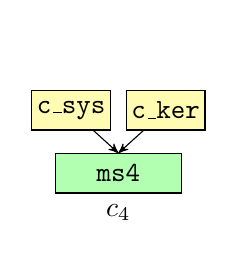
\begin{tikzpicture}[->,>=stealth']

  \node[rectangle,
        draw,
        fill = green!30,
        minimum width = 1.6cm, 
        minimum height = 0.5cm
        ] (ms4) at (0,0) {};
  \node[] at (ms4.center) {\texttt{ms4}};

  \node[rectangle,
  minimum width = 1cm, 
  minimum height = 0.5cm
  ] (lab) at (0,-.5) {};
\node[] at (lab.center) {$c_4$};

  %\node[rectangle,
  %    draw,
  %    minimum width = 1.5cm, 
  %    minimum height = 0.5cm
  %    ] (ms) at (-1,1) {};
  %\node[] at (ms.center) {ms};

  \node[rectangle,
      draw,
      fill = yellow!30,
      minimum width = 1cm, 
      minimum height = 0.5cm
      ] (ker) at (.6,.8) {};
  \node[] at (ker.center) {\texttt{c\_ker}};

  \node[rectangle,
      draw,
      fill = yellow!30,
      minimum width = 1cm, 
      minimum height = 0.5cm
      ] (sys) at (-.6,.8) {};
  \node[] at (sys.center) {\texttt{c\_sys}};

  \node[rectangle,
      minimum width = 1cm, 
      minimum height = 0.5cm
      ] (ms3) at (.6,1.6) {};
  \node[] at (ms3.center) {};

%     \node[rectangle,
%     minimum width = 1cm, 
%     minimum height = 0.5cm
%     ] (label) at (0,-0.5) {};
% \node[] at (label.center) {m3b};


  \path[every node/.style={font=\sffamily\small}]
  %host1 path
  (ker) edge [] node [right] {} (ms4.north)
  (sys) edge [] node [right] {} (ms4.north) ;
  % (ms) edge [] node [right] {} (ms4.north) ;


\end{tikzpicture} 
                & \input{examples/rtm_ker-vc-sys-seq_reduced-copy/m3.tex} 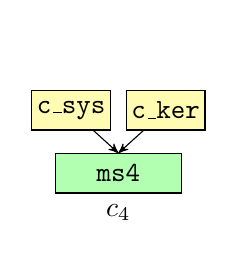
\begin{tikzpicture}[->,>=stealth']

  \node[rectangle,
        draw,
        fill = green!30,
        minimum width = 1.6cm, 
        minimum height = 0.5cm
        ] (ms4) at (0,0) {};
  \node[] at (ms4.center) {\texttt{ms4}};

  \node[rectangle,
  minimum width = 1cm, 
  minimum height = 0.5cm
  ] (lab) at (0,-.5) {};
\node[] at (lab.center) {$c_4$};

  %\node[rectangle,
  %    draw,
  %    minimum width = 1.5cm, 
  %    minimum height = 0.5cm
  %    ] (ms) at (-1,1) {};
  %\node[] at (ms.center) {ms};

  \node[rectangle,
      draw,
      fill = yellow!30,
      minimum width = 1cm, 
      minimum height = 0.5cm
      ] (ker) at (.6,.8) {};
  \node[] at (ker.center) {\texttt{c\_ker}};

  \node[rectangle,
      draw,
      fill = yellow!30,
      minimum width = 1cm, 
      minimum height = 0.5cm
      ] (sys) at (-.6,.8) {};
  \node[] at (sys.center) {\texttt{c\_sys}};

  \node[rectangle,
      minimum width = 1cm, 
      minimum height = 0.5cm
      ] (ms3) at (.6,1.6) {};
  \node[] at (ms3.center) {};

%     \node[rectangle,
%     minimum width = 1cm, 
%     minimum height = 0.5cm
%     ] (label) at (0,-0.5) {};
% \node[] at (label.center) {m3b};


  \path[every node/.style={font=\sffamily\small}]
  %host1 path
  (ker) edge [] node [right] {} (ms4.north)
  (sys) edge [] node [right] {} (ms4.north) ;
  % (ms) edge [] node [right] {} (ms4.north) ;


\end{tikzpicture}  \\
                 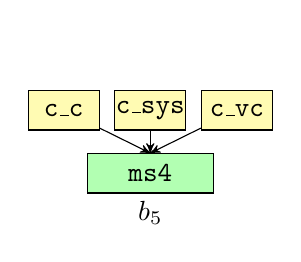
\begin{tikzpicture}[->,>=stealth']

    \node[rectangle,
          draw,
          fill = green!30,
          minimum width = 1.6cm, 
          minimum height = 0.5cm
          ] (ms4) at (0,0) {};
    \node[] at (ms4.center) {\texttt{ms4}};

    \node[rectangle,
    minimum width = 1cm, 
    minimum height = 0.5cm
    ] (lab) at (0,-.5) {};
  \node[] at (lab.center) {$b_5$};

    \node[rectangle,
        draw,
        fill = yellow!30,
        minimum width = .9cm, 
        minimum height = 0.5cm
        ] (vc) at (1.1,.8) {};
    \node[] at (vc.center) {\texttt{c\_vc}};

    \node[rectangle,
        draw,
        fill = yellow!30,
        minimum width = .9cm, 
        minimum height = 0.5cm
        ] (c) at (-1.1,.8) {};
    \node[] at (c.center) {\texttt{c\_c}};

    \node[rectangle,
        draw,
        fill = yellow!30,
        minimum width = .9cm, 
        minimum height = 0.5cm
        ] (sys) at (0,.8) {};
    \node[] at (sys.center) {\texttt{c\_sys}};

    \node[rectangle,
        minimum width = .9cm, 
        minimum height = 0.5cm
        ] (ms3) at (1.1,1.6) {};
    \node[] at (ms3.center) {};


    \path[every node/.style={font=\sffamily\small}]
    %host1 path
    (vc) edge [] node [right] {} (ms4.north)
    (c) edge [] node [right] {} (ms4.north)
    (sys) edge [] node [right] {} (ms4.north) ;
    % (ms) edge [] node [right] {} (ms4.north) ;


\end{tikzpicture}
                 & 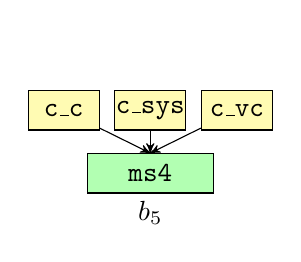
\begin{tikzpicture}[->,>=stealth']

    \node[rectangle,
          draw,
          fill = green!30,
          minimum width = 1.6cm, 
          minimum height = 0.5cm
          ] (ms4) at (0,0) {};
    \node[] at (ms4.center) {\texttt{ms4}};

    \node[rectangle,
    minimum width = 1cm, 
    minimum height = 0.5cm
    ] (lab) at (0,-.5) {};
  \node[] at (lab.center) {$b_5$};

    \node[rectangle,
        draw,
        fill = yellow!30,
        minimum width = .9cm, 
        minimum height = 0.5cm
        ] (vc) at (1.1,.8) {};
    \node[] at (vc.center) {\texttt{c\_vc}};

    \node[rectangle,
        draw,
        fill = yellow!30,
        minimum width = .9cm, 
        minimum height = 0.5cm
        ] (c) at (-1.1,.8) {};
    \node[] at (c.center) {\texttt{c\_c}};

    \node[rectangle,
        draw,
        fill = yellow!30,
        minimum width = .9cm, 
        minimum height = 0.5cm
        ] (sys) at (0,.8) {};
    \node[] at (sys.center) {\texttt{c\_sys}};

    \node[rectangle,
        minimum width = .9cm, 
        minimum height = 0.5cm
        ] (ms3) at (1.1,1.6) {};
    \node[] at (ms3.center) {};


    \path[every node/.style={font=\sffamily\small}]
    %host1 path
    (vc) edge [] node [right] {} (ms4.north)
    (c) edge [] node [right] {} (ms4.north)
    (sys) edge [] node [right] {} (ms4.north) ;
    % (ms) edge [] node [right] {} (ms4.north) ;


\end{tikzpicture} \\ 
            \end{tabular}
    \end{center}
    \caption{Normalized attack trees for $P1$ and $P2$}
    \label{fig:rtm-compare-reduced}
\end{figure}

%% TODO: Elaborate on why individual tree ordering relationships hold
Now, let us first compare the first and second protocols. We begin by collecting the Chase output and reducing the attack trees to normal form as shown in Figure \ref{fig:rtm-compare-reduced}. Next, we can determine the ordering relationships between the individual attack trees in the two sets: $a_1 \simeq b_1$, $a_2 \simeq b_2$, $a_3 \prec b_3$, $a_4 \prec b_4$, and $a_5 \simeq b_5$. Lastly we can determine the ordering relationships between the two protocols. It is clear to see that for every attack $b$ in $P2$ there exists an attack $a$ in $P1$ such that $a \preceq b$. Therefore, we can conclude that $P1 \leq P2$. Furthermore, it is not the case that $P2 \leq P1$ since there is no attack in $P2$ that is less than $a_3$ or $a_4$. Our ultimate conclusion supports hypothesis 1 that measurements that mimic the system's dependency chain better confine the adversary.

%% TODO: Elaborate on why individual tree ordering relationships hold
%% TODO: Elaborate on antisymmetry application
Next, let us compare the first and third protocols. The set of reduced
attack trees for the third protocol is shown in Figure
\ref{fig:hv-reduced}. Now we can determine the ordering relationships
between the individual attack trees in the two sets: $a_1 \simeq c_1$,
$a_2 \simeq c_2$, $a_3 \simeq c_3$, $a_4 \simeq c_4$, $a_5 \simeq
c_5$, $a_2 \simeq c_6$, $a_1 \prec c_7$, $a_2 \prec c_8$, $a_4 \prec
c_9$, and $a_5 \prec c_{10}$. And again lastly we can determine the
ordering relationships between the two protocols: $P1 \leq P3$ and $P3
\leq P1$. Therefore, by the antisymmetry property of our partial
order, we can conclude that these two protocols have the same set of
weakest attacks, namely $\{a_1, a_3, a_5\}$ and $\{c_1, c_3,
c_5\}$. This proves hypothesis 2 that increasing the number of
measurements does not necessarily further confine the adversary. 


\begin{figure}[h]
  \begin{center}
      \begin{tabular}{ M{5.2cm} M{6.8cm} }
              \multicolumn{2}{c}{$P3$} \\
              \hline
              \\
              \input{examples/ker_vs-hv-sys-seq_reduced/m1.tex} \hspace{.03cm} 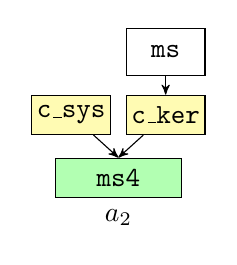
\begin{tikzpicture}[->,>=stealth']

    \node[rectangle,
          draw,
          fill = green!30,
          minimum width = 1.6cm, 
          minimum height = 0.5cm
          ] (ms4) at (0,0) {};
    \node[] at (ms4.center) {\texttt{ms4}};

    \node[rectangle,
    minimum width = 1cm, 
    minimum height = 0.5cm
    ] (lab) at (0,-.5) {};
  \node[] at (lab.center) {$a_2$};

    \node[rectangle,
        draw,
        fill = yellow!30,
        minimum width = 1cm, 
        minimum height = 0.5cm
        ] (sys) at (-.6,.8) {};
    \node[] at (sys.center) {\texttt{c\_sys}};

    \node[rectangle,
        draw,
        fill = yellow!30,
        minimum width = 1cm, 
        minimum height = 0.5cm
        ] (vc) at (.6,.8) {};
    \node[] at (vc.center) {\texttt{c\_ker}};

    \node[rectangle,
        draw,
        minimum width = 1cm, 
        minimum height = 0.6cm
        ] (ms3) at (.6,1.6) {};
    \node[] at (ms3.center) {\texttt{ms}};

%     \node[rectangle,
%     minimum width = 1cm, 
%     minimum height = 0.5cm
%     ] (label) at (0,-0.5) {};
% \node[] at (label.center) {m2b};


    \path[every node/.style={font=\sffamily\small}]
    %host1 path
    (ms3) edge [] node [right] {} (vc.north)
    (vc) edge [] node [right] {} (ms4.north) 
    (sys) edge [] node [right] {} (ms4.north) ;


\end{tikzpicture} & 
              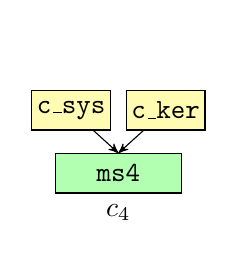
\begin{tikzpicture}[->,>=stealth']

  \node[rectangle,
        draw,
        fill = green!30,
        minimum width = 1.6cm, 
        minimum height = 0.5cm
        ] (ms4) at (0,0) {};
  \node[] at (ms4.center) {\texttt{ms4}};

  \node[rectangle,
  minimum width = 1cm, 
  minimum height = 0.5cm
  ] (lab) at (0,-.5) {};
\node[] at (lab.center) {$c_4$};

  %\node[rectangle,
  %    draw,
  %    minimum width = 1.5cm, 
  %    minimum height = 0.5cm
  %    ] (ms) at (-1,1) {};
  %\node[] at (ms.center) {ms};

  \node[rectangle,
      draw,
      fill = yellow!30,
      minimum width = 1cm, 
      minimum height = 0.5cm
      ] (ker) at (.6,.8) {};
  \node[] at (ker.center) {\texttt{c\_ker}};

  \node[rectangle,
      draw,
      fill = yellow!30,
      minimum width = 1cm, 
      minimum height = 0.5cm
      ] (sys) at (-.6,.8) {};
  \node[] at (sys.center) {\texttt{c\_sys}};

  \node[rectangle,
      minimum width = 1cm, 
      minimum height = 0.5cm
      ] (ms3) at (.6,1.6) {};
  \node[] at (ms3.center) {};

%     \node[rectangle,
%     minimum width = 1cm, 
%     minimum height = 0.5cm
%     ] (label) at (0,-0.5) {};
% \node[] at (label.center) {m3b};


  \path[every node/.style={font=\sffamily\small}]
  %host1 path
  (ker) edge [] node [right] {} (ms4.north)
  (sys) edge [] node [right] {} (ms4.north) ;
  % (ms) edge [] node [right] {} (ms4.north) ;


\end{tikzpicture} \hspace{.03cm} \input{examples/ker_vs-hv-sys-seq_reduced/m6.tex} \\
              \multirow{4}{*}[.45cm]{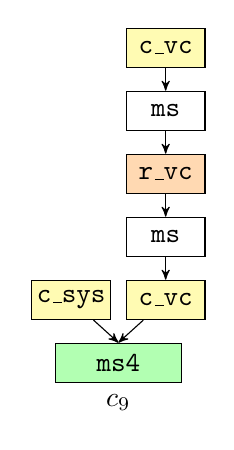
\begin{tikzpicture}[->,>=stealth']

    \node[rectangle,
          draw,
          fill = green!30,
          minimum width = 1.6cm, 
          minimum height = 0.5cm
          ] (ms4) at (0,0) {};
    \node[] at (ms4.center) {\texttt{ms4}};

    \node[rectangle,
    minimum width = 1cm, 
    minimum height = 0.5cm
    ] (lab) at (0,-.5) {};
  \node[] at (lab.center) {$c_9$};
  

    \node[rectangle,
        draw,
        fill = yellow!30,
        minimum width = 1cm, 
        minimum height = 0.5cm
        ] (sys) at (-.6,.8) {};
    \node[] at (sys.center) {\texttt{c\_sys}};

    \node[rectangle,
        draw,
        fill = yellow!30,
        minimum width = 1cm, 
        minimum height = 0.5cm
        ] (vc) at (.6,.8) {};
    \node[] at (vc.center) {\texttt{c\_vc}};

    \node[rectangle,
        draw,
        minimum width = 1cm, 
        minimum height = 0.5cm
        ] (ms3) at (.6,1.6) {};
    \node[] at (ms3.center) {\texttt{ms}};
    
    \node[rectangle,
    draw,
    fill = orange!30,
    minimum width = 1cm, 
    minimum height = 0.5cm
    ] (rvc) at (.6,2.4) {};
    \node[] at (rvc.center) {\texttt{r\_vc}};

    \node[rectangle,
        draw,
        minimum width = 1cm, 
        minimum height = 0.5cm
        ] (ms2) at (.6,3.2) {};
    \node[] at (ms2.center) {\texttt{ms}};

    \node[rectangle,
        draw,
        fill = yellow!30,
        minimum width = 1cm, 
        minimum height = 0.5cm
        ] (cvc) at (.6,4) {};
    \node[] at (cvc.center) {\texttt{c\_vc}};

    \path[every node/.style={font=\sffamily\small}]
    %host1 path
    (ms3) edge [] node [right] {} (vc.north)
    (vc) edge [] node [right] {} (ms4.north) 
    (sys) edge [] node [right] {} (ms4.north) 
    (rvc) edge [] node [right] {} (ms3.north)
    (ms2) edge [] node [right] {} (rvc.north)
    (cvc) edge [] node [right] {} (ms2.north);


\end{tikzpicture} \hspace{.03cm} \input{examples/ker_vs-hv-sys-seq_reduced/m10.tex}} & 
              \input{examples/ker_vs-hv-sys-seq_reduced/m8.tex} \hspace{.03cm} \input{examples/ker_vs-hv-sys-seq_reduced/m3.tex} \\
              & \\
              & 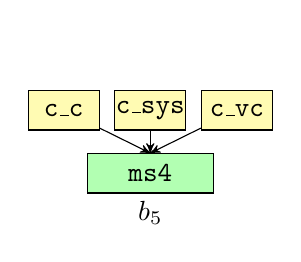
\begin{tikzpicture}[->,>=stealth']

    \node[rectangle,
          draw,
          fill = green!30,
          minimum width = 1.6cm, 
          minimum height = 0.5cm
          ] (ms4) at (0,0) {};
    \node[] at (ms4.center) {\texttt{ms4}};

    \node[rectangle,
    minimum width = 1cm, 
    minimum height = 0.5cm
    ] (lab) at (0,-.5) {};
  \node[] at (lab.center) {$b_5$};

    \node[rectangle,
        draw,
        fill = yellow!30,
        minimum width = .9cm, 
        minimum height = 0.5cm
        ] (vc) at (1.1,.8) {};
    \node[] at (vc.center) {\texttt{c\_vc}};

    \node[rectangle,
        draw,
        fill = yellow!30,
        minimum width = .9cm, 
        minimum height = 0.5cm
        ] (c) at (-1.1,.8) {};
    \node[] at (c.center) {\texttt{c\_c}};

    \node[rectangle,
        draw,
        fill = yellow!30,
        minimum width = .9cm, 
        minimum height = 0.5cm
        ] (sys) at (0,.8) {};
    \node[] at (sys.center) {\texttt{c\_sys}};

    \node[rectangle,
        minimum width = .9cm, 
        minimum height = 0.5cm
        ] (ms3) at (1.1,1.6) {};
    \node[] at (ms3.center) {};


    \path[every node/.style={font=\sffamily\small}]
    %host1 path
    (vc) edge [] node [right] {} (ms4.north)
    (c) edge [] node [right] {} (ms4.north)
    (sys) edge [] node [right] {} (ms4.north) ;
    % (ms) edge [] node [right] {} (ms4.north) ;


\end{tikzpicture} \hspace{.03cm} 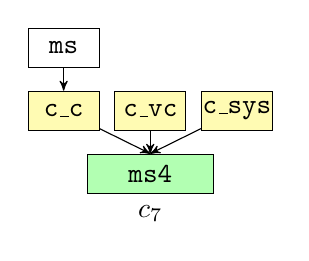
\begin{tikzpicture}[->,>=stealth']

  \node[rectangle,
        draw,
        fill = green!30,
        minimum width = 1.6cm, 
        minimum height = 0.5cm
        ] (ms4) at (0,0) {};
  \node[] at (ms4.center) {\texttt{ms4}};

  \node[rectangle,
  minimum width = 1cm, 
  minimum height = 0.5cm
  ] (lab) at (0,-.5) {};
\node[] at (lab.center) {$c_7$};

  \node[rectangle,
      draw,
      fill = yellow!30,
      minimum width = .9cm, 
      minimum height = 0.5cm
      ] (sys) at (-1.1,.8) {};
  \node[] at (sys.center) {\texttt{c\_c}};

  \node[rectangle,
      draw,
      fill = yellow!30,
      minimum width = .9cm, 
      minimum height = 0.5cm
      ] (ker) at (1.1,.8) {};
  \node[] at (ker.center) {\texttt{c\_sys}};

  \node[rectangle,
      draw,
      fill = yellow!30,
      minimum width = .9cm, 
      minimum height = 0.5cm
      ] (vc) at (0,.8) {};
  \node[] at (vc.center) {\texttt{c\_vc}};

  \node[rectangle,
      draw,
      minimum width = .9cm, 
      minimum height = 0.5cm
      ] (ms1) at (-1.1,1.6) {};
  \node[] at (ms1.center) {\texttt{ms}};

  %\node[rectangle,
  %    draw,
  %    minimum width = 1.5cm, 
  %    minimum height = 0.5cm
  %    ] (ms2) at (-1,1) {};
  %\node[] at (ms2.center) {ms'};

%     \node[rectangle,
%     minimum width = 1.5cm, 
%     minimum height = 0.5cm
%     ] (label) at (0,-0.5) {};
% \node[] at (label.center) {m4c};


  \path[every node/.style={font=\sffamily\small}]
  %host1 path
  (ms1) edge [] node [right] {} (sys.north)
  (ker) edge [] node [right] {} (ms4.north)
  (vc) edge [] node [right] {} (ms4.north)
  % (ms2) edge [] node [right] {} (ms4.north) 
  (sys) edge [] node [right] {} (ms4.north) ;


\end{tikzpicture} \\
              & \\
          \end{tabular}
  \end{center}
  \caption{Normalized attack trees for $P3$}
  \label{fig:hv-reduced}
\end{figure}

These examples demonstrate the applicability of our ordering approach
to examples from the literature. With these completed examples, we
reliably conclude our protocol ordering methodology successfully
enhances the evaluation of remote attestation protocols. Leveraging
the Chase model finder, we order Copland protocols according to their
adversary constraint by comparing all possible attack trees and
linking the relationship between attack trees to the protocol in
question. 

\section{Conclusion}
%% TODO: Conclusion

Remote attestation is a process of gathering and appraising evidence
reflecting a system's behavior.  Attacks on remote attestation include
attempts to hide nefarious behavior by corrupting and repairing
components in a way that avoids detection.  Inspired by
\citet{Rowe:2021:OnOrdering} and using the Chase model
finder~\citep{Ramsdell:2020:Chase} we have developed and verified a
partial ordering for attestation protocols.  This ordering reflects
relative resistance to attack.  We say that $P_0\leq P_1$ if avoiding
detection by $P_1$ is at least as hard as $P_0$ based on comparing
allowed attacks.

Our ordering is useful as a static design metric and a dynamic
negotiation metric.  During protocol design ordering helps establish
when design changes truly impact the quality or strength of a
protocol.  During protocol negotiation~\citep{Fritz:2023:framework}
the ordering allows an appraiser to choose a best protocol from a
proposal generated by a target.

Next up is looking at the quality of individual measurements.  This
work examined only measurement event ordering without consideration of
what evidence measurements gather.  We are now working on techniques for
evaluating individual and composite measurement quality that will
integrate with this work, ultimately providing a mechanism for fully
comparing and assessing the quality of attestation protocols.




%%%%%%%%%%%
% Quick and dirty example using \verb+listings+ to format Coq code:

% \begin{lstlisting}[language=coq]
%   Definition x:nat := 3.
%   Fixpoint f(x:nat):nat := if x=0 then 1 else x*f(x-1).
% \end{lstlisting}

%
% 
% ---- Bibliography ----
%
% BibTeX users should specify bibliography style 'splncs04'.
% References will then be sorted and formatted in the correct style.
%
%\bibliographystyle{splncs04}
\bibliographystyle{splncsnat}
%\bibliography{sldg}
\bibliography{works}
%
\end{document}
